\section{OpenStreetMap}
As mentioned in the introduction, one of the main actors discussed in this paper is \textit{OpenStreetMap} (\textit{OSM})\cite{haklay2008openstreetmap}, a powerful platform in continuous evolution that relies on a strong and passionate community, which is the one of the best worldwide representation of a crowdsourced project\cite{chilton2009crowdsourcing}.
OSM is an open-source project, started in 2004, with the aim of collect and freely provide geospatial data to anyone.

\subsection{Parties inside the organization}
The \textit{foundation} (OSMF) that stands beside the project is an international non-profit that wants to follow the developments of the project, encouraging the growth and distribution without controlling or managing OSM. It's important to emphasize that the community is the heart of the project, leading the entire development process.

\textit{Volunteers} are organized in development groups, even if the components decided to participate for such different goals: for someone can be an hobby, for others it's just a matter of enriching a particular area that they evaluate as relevant, but there's space also for who thinks that OSM could be crucial in case of geological crisis such as earthquakes and tsunamis.

\textit{Groups} are used to organize the so-called ``\textit{mapping parties}'', in which volunteers meet each other with the aim of mapping all together a specific uncovered area. These events are also the springboard to attract new volunteers who espouse the cause and, for sure, instruct them on how the OSM's process works.

It's impressive to see how the effort behind the project is spread between such different realities: as well explained in \cite{haklay2008openstreetmap}, the OSM community is composed by passionate individuals but they're supported by different organizations such as states and even different private companies.

\subsection{Growth and diffusion}
Nowadays OSM is one of the reference points for geospatial services, along with Google Maps, Bing Maps and MapBox. Although the project was launched in the first lustrum of 2000, it experienced strong growth in the first half of 2012.
In fact, us reported by BBC\footnote{Google Maps to charge for usage, \href{https://www.bbc.com/news/business-15523050}{BBC}, 31 October 2011.}, Google announced in October 2011 the intent to introduce a fee for services that rely on Google Maps API, starting from April 2012. Going deeper into the details, the fee is only charged for services that make intensive use of the API, recording more than 25,000 map hits per day. Together with the announce, Google reported that, according to their projections, only 0,35\% of users would have been involved in the tariff change. Google has reserved the right to publish the real impact of their policy, leaving to this percentage irrelevant importance from a statistical point of view, but rather just using it for the marketing side.
What is important after the actuation of this policy is the effects that have been generated for the competitors: OSM gained the most, thanks to his accuracy and, most important, his concept of open-source data.
The growth can be supported by the graph in figure \ref{fig:osm_users}\footnote{OpenStreetMap Wiki, \href{https://wiki.openstreetmap.org/wiki/Stats}{Stats section}.}, in which is easy to notice how many users started to join the community, establishing a positive trend that still today seems to be constantly growing.
It's interesting to notice how companies that push on open source philosophy, as well as others that do not, decided to migrate to OSM.
Wikipedia was one of the first organizations that jumped in\footnote{Wikipedia updates mobile apps, drops Google Maps for OpenStreetMap, \href{https://www.theverge.com/2012/4/7/2931320/wikipedia-updates-mobile-apps-drops-google-maps-for-openstreetmap}{TheVerge}, 7 April 2012.}: for obvious reasons, the two sides find many points of contact, where surely emerges the concept of community on which the two services are based.

Even private companies decided to trust the open-source movement, adopting OSM after years of Google Maps usage: this is the case of Foresquare and StreetEasy\footnote{After price hike, Foursquare and StreetEasy switch from Google to OpenStreetMaps, \href{https://venturebeat.com/2012/03/01/google-maps-api-price-foursquare-streeteasy-openstreetmaps/}{VentureBeat}, 1 March 2012.}, which decided to migrate in favor of the open service, with a higher level of customization and design flexibility.

Today OpenStreetMap is used by many huge companies such as Facebook, Amazon, Apple, Microsoft, Pinterest, Snapchat and Uber as well as so many different governments, universities (Cambridge is just one instance) and news and media agencies\footnote{OpenStreetMap Wiki, \href{https://welcome.openstreetmap.org/about-osm-community/consumers/}{Who uses OpenStreetMap?}}.

\begin{figure}
    \centering
    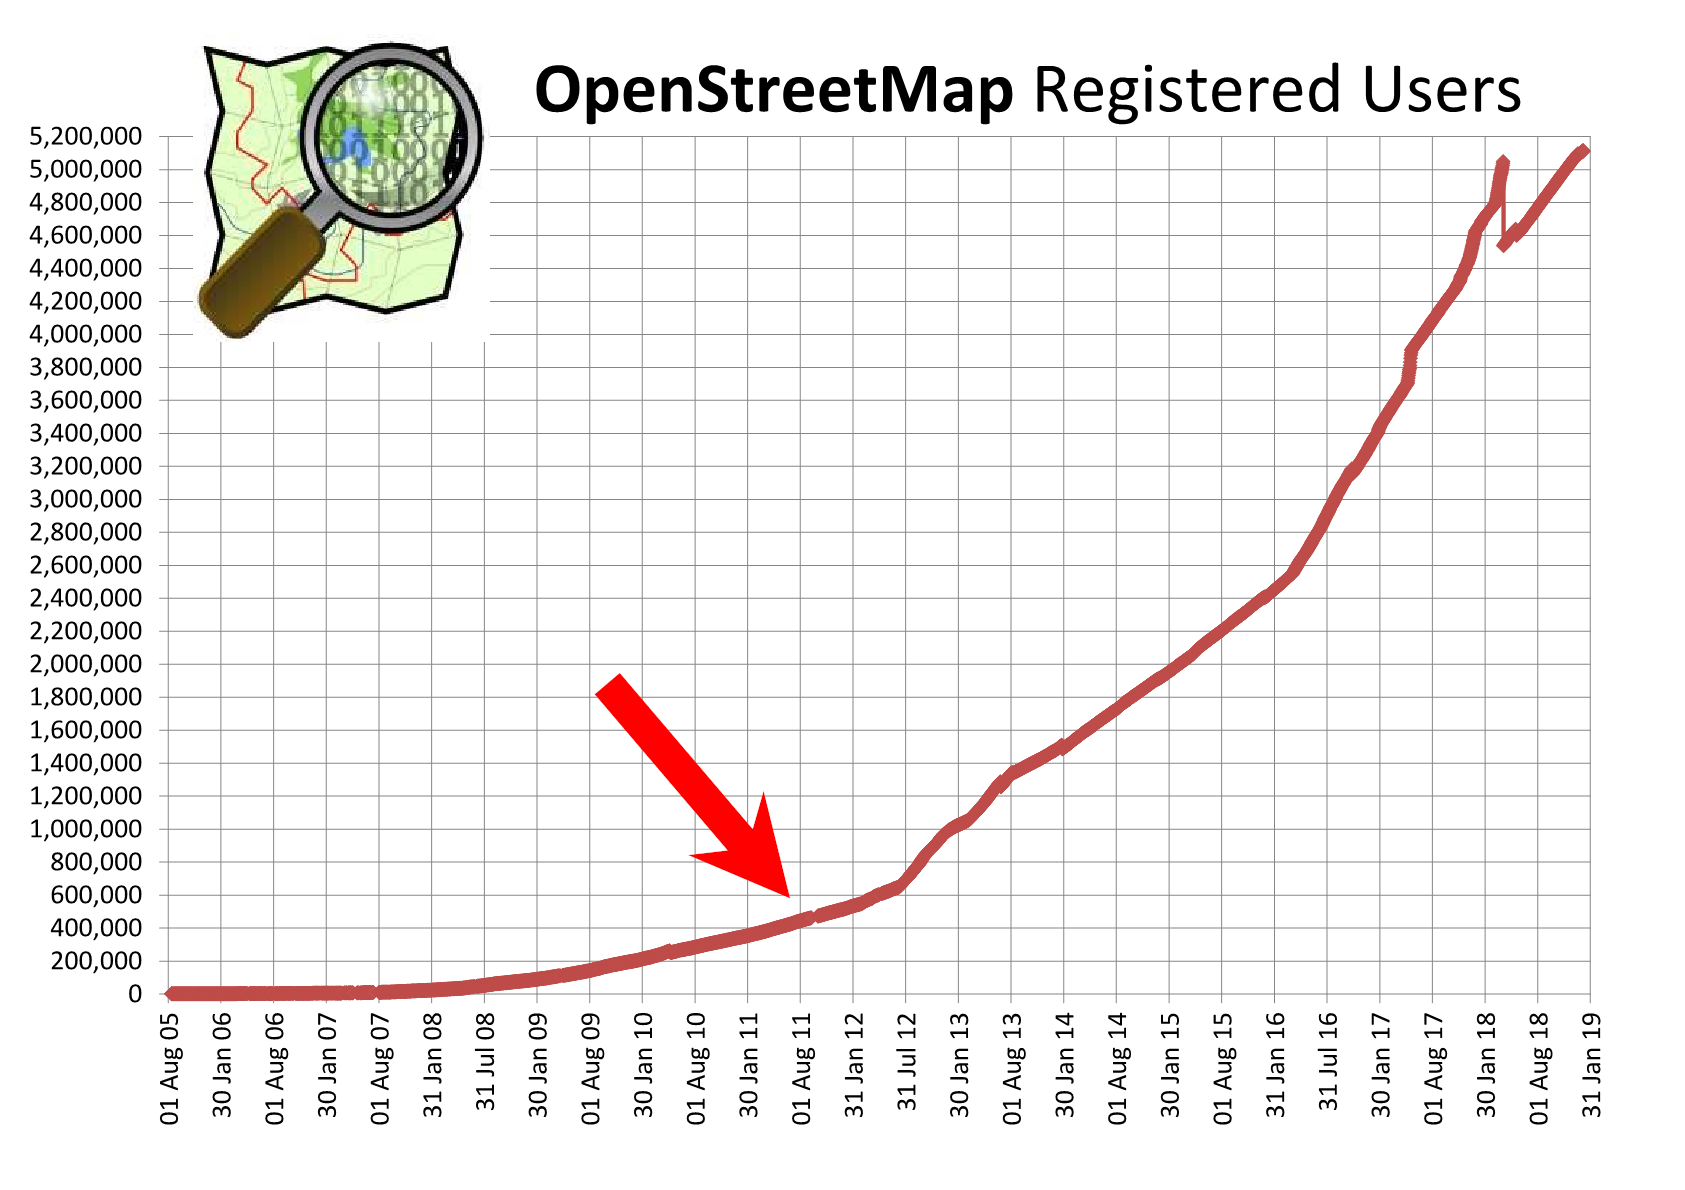
\includegraphics[width=0.9\linewidth]{images/osm_registered_users.png}
    \caption{OSM Accumulated registered users}
    \label{fig:osm_users}
\end{figure}

Another relevant point of discussion is the accuracy and coverage of the mapping data across different services, all with the same purpose. Different approaches has been studied to understand points of divergence and causes that stand behind those. 5 different cities in Ireland have been taken into account in a study\cite{ciepluch2010comparison}. The paper outcome is noteworthy: in comparison, Google Maps and OSM accuracy seems to be equal, underlining how far a community-based project can go. The sticking point of the comparison is the coverage: important areas are well-mapped, but, differently
from Google Maps, OSM lack in peripheral coverage.
The author of the study used to describe the phenomenon as ``\textit{areas where nobody wants to map}". In fact, this description traces perfectly where the point of the discussion is: Google has a relevant advantage with respect to OSM because is a private organization that doesn't rely on the community's needs.
This problem has been noticed also by Caquard S.\cite{caquard2014cartographyII}, which states that, despite the significant improvement that mapping communities have made over the years, inequalities persist in terms of geospatial contribution.
This is still representing the major obstacle for OSM development in the long run.

\subsection{Imports}
Before digging into adopted licenses and related issues, is worthy to analyze how new data is processed in order to be inserted into the database, and consequently, be available for the final user.

\subsubsection{Control entities: DWG \& LWG}~\\ \newline
In the \textit{import} process, two entities, both authorized by the OSMF, play crucial roles:
\begin{itemize}
    \item The \textbf{Data Working Group}\footnote{\href{https://wiki.osmfoundation.org/wiki/Data_Working_Group}{DWG official wiki}.} (DWG) is the authority that provides integrity on stored data. It handles user's complaints and regulates discussions and disputes that can come up in decisions taken by the community. It also has decision-making power in case of vandalism detection, asking to the \textit{Operations Working Group} (OWG) to ban or limit the usage of APIs for a certain IP address and even deleting all diary entities.
    \item The \textbf{Licensing Working Group}\footnote{\href{https://wiki.osmfoundation.org/wiki/Licensing_Working_Group}{LWG official wiki}.} (LWG) is responsible for all licensing issues related to geodata: creation of new contents, following the \textit{import} process, need to be regulated and pass through licensing controls, as well as correct usages of provided information (end-user license).
    The team is also in charge of handling possible copyright infringement raised by intellectual property owners, as well as all other possible disputes such as child protection, privacy, trademarks and so on.
\end{itemize}
OSM is composed by some other working groups that are missing here, but since these two are the most important ones for this work, it's been decided to overcome the description of each group that composes the organization.
By the way, it's important to notice that all the different groups are always composed by a restricted number of community members that for a long time have contributed to the development of the project.

\subsubsection{Import processing}~\\ \newline
The \textit{Import} is the procedure to follow by which community can add their contributes in the database.
At first, it's hardly recommended to discuss with the community before start working on the data collection: a certain kind of information could be useful in a specific area, rather than in another city in which is not relevant at all. It's important to notice that the community (distributed inside a hierarchical organization, starting from countries till local groups) should approve your plan and can simply deny accepting the submitted work at this very first stage.
Depending on the complexity and scale of the import, the DWG can ask for technical assistance of some experienced OSM volunteers.
After passing this early stage, license approval needs to be taken into account. Permissions and licenses need to be obtained from the data owner. Most important, all licenses need to be complied with \textit{Open Database License} (ODbL) in order to be uploaded and used in OSM platform (more on ODbL in section \ref{sec:licensechange}).  
This is a crucial point of interest for this study: obtain licenses, in most of the cases, appears to be the hardest task to be accomplished because of policies that may be in use depending on localities and organizations. Still, this one of the main reason why the majority of license conflicts came out. Policies can be almost open but still having conflicts or, for instance, could have restrictions for commercial use or attribution requirements.
The LWG, as the guarantor of this delicate phase, provides volunteers with templates to expressly request to data owners if they are willing to comply with the OSM ODbL terms.
After accomplishing this awkward phase, the volunteer must document how he is planning to complete the import. Raw data need to be converted into OSM XML format and be handled in such a way that permit to simplify and, at the same time, be more informative as possible. The user is not alone and should mention in the documentation other volunteers to split the work.
Before start the provided plan, the documentation needs to be submitted for the final review, made by different delegations of the foundation (of course DWG and LWG take part in the review). Only when a confirmation will be sent back, the import can be finalized realizing the plan, tracking progresses to the community till the end of all the procedures.